\documentclass[aspectratio=169]{beamer}

\usepackage{tabularx}
\usepackage{booktabs}
\usepackage{colortbl}
\usepackage{media9}
\usepackage{multimedia}
\usepackage{hyperref}
\usepackage{subfigure}
% \usepackage[brazil]{babel}
\usepackage{amssymb}
\usepackage{amsthm,amsfonts}
\usepackage[utf8]{inputenc}
\usepackage{latexsym}
\usepackage{float}
\usepackage[T1]{fontenc}
\usepackage{beamerthemeshadow}
\usepackage{helvet}
\usepackage{graphicx}       % I don't think color.sty is needed.
\usepackage{epstopdf}
\usepackage{listings}
\usepackage{tikz}
\usetikzlibrary{arrows,shapes}
\usepackage{algpseudocode}
\usepackage{algorithm}
\usepackage{algorithmicx}
\usepackage{subfigure}
% \usepackage[brazil]{babel}
\usepackage{amssymb}
\usepackage{amsthm,amsfonts}
\usepackage[utf8]{inputenc}
\usepackage{latexsym}
\usepackage{float}
\usepackage{beamerthemeshadow}
\usepackage{lipsum}
\usepackage{listings}
\usepackage{color}
\usepackage{xcolor}
\usepackage{tikz}
\usetikzlibrary{arrows,shapes}
\usepackage{color, colortbl}
\usepackage{float} 
\floatplacement{figure}{hb} 
\floatplacement{table}{hb} 
\usepackage{placeins} 
\definecolor{Gray}{gray}{0.9}
\usepackage{stfloats}
\usepackage{tabularx}
\usepackage{fancyhdr}

\addmediapath{.}

%  \usetheme{Copenhagen}
\usetheme{Darmstadt}
%    \usetheme{default}
% \usetheme{Antibes}

% \usecolortheme{crane}
\usecolortheme{default}
% \usecolortheme{dolphin}
% \usecolortheme{seagull}
% \usecolortheme{seahorse}

\newcommand{\mc}[2]{\multicolumn{#1}{c}{#2}}
\definecolor{Gray}{gray}{0.85}
\definecolor{LightCyan}{rgb}{0.7,1,1}\setbeamersize{text margin left=10pt,text margin right=10pt}

\newcolumntype{a}{>{\columncolor{Gray}}c}\setbeamertemplate{footline}[frame number]
\newcolumntype{b}{>{\columncolor{white}}c}
\beamertemplatetransparentcovereddynamic

\AtBeginSection[]
{
   \begin{frame}
   \frametitle{Outline}
       \tableofcontents[currentsection]
   \end{frame}
}

\setbeamercolor{block body}{bg=blue!22,fg=black}

\begin{document}

\title[]{\textbf{MODELO ADAPTATIVO PARA PREVISÃO DE DEMANDA POR RECURSOS DE REDE EM PROVEDORES DE INTERNET MODERNOS}}  

\author[Dyego Oliveira]{Dyego Henrique Leonel Oliveira}

\institute{Universidade Estadual do Ceará (UECE)}

\date{Julho 2020} 

\begin{frame}
\titlepage

\end{frame}

% \setcounter{tocdepth}{1}

\begin{frame}
\frametitle{Outline }
\tableofcontents
\end{frame} 

%%%%%%%%%%%%%%%%%%%%%%%%%%%%%%%%%%%%%%
%-------------------------------------
%%%%%%%%%%%%%%%%%%%%%%%%%%%%%%%%%%%%%%

\section{Introdução}

%%%%%%%%%%%%

\subsection{}
\begin{frame}
\frametitle{Introdução}
% \small
\begin{block}{Contexto}
    \begin{itemize}
        \item A Internet tem se tornado uma ferramenta crucial em nossas vidas, pelos serviços modernos de comptuação que operam sobre.
        \item A maioria desses serviços são baseados em:
        \begin{itemize}
            \item Service Level Agreement -- SLA
            \item Internet Access Service -- IAS
        \end{itemize}
        \item Operando através o Internet Service Provider (ISP)
    \end{itemize}
\end{block}


\end{frame}
%%%%%%%%%%%%
\subsection{}
\begin{frame}{Introdução}
    \begin{block}{Desafios}
\begin{itemize}
    \item Todos os tipos de redes buscam por características tais como:
    \begin{itemize}\setbeamertemplate{itemize items}[triangle]
        \item baixo atraso;
        \item flexibilidade;
        \item resiliência;
    \end{itemize}
    \item Pontos necessários para evoluir o gerenciamento de recursos, flexibilidade, bandwidth e poder personalizar o comportamento de infraestruturas das redes.
\end{itemize}
\end{block}
\end{frame}
%%%%%%%%%%%%

\subsection{}
\begin{frame}
\frametitle{Introdução}
% \small
\begin{block}{MISPs e Demanda Elastica}
    \begin{itemize}
    \item ISPs tendem a evoluir para MISPs (Modern Internet Service Providers), abordando situações como demanda elástica por recursos de rede. 
    \item Os MISPs precisam expandir ou reduzir dinamicamente a alocação de largura de banda (comportamento elástico), permitindo um IAS adequado sob demanda. Evitando problemas de lentidão, interrupção e desconecções. 
    \item Uma abordagem promissora para os MISPs são o desenvolvimento de fatias de redes (slices). Cada fatia pode ter a configuração adequada para melhor atender as necessidades do cliente.
    \item Uma abordagem promisora para lidar com (slices) é o uso de Previsão de Tráfego de Rede.
    \end{itemize}
\end{block}
\end{frame}

%%%%%%%%%%%%

\subsection{}
\begin{frame}
\frametitle{Introdução}
% \small
\begin{block}{Modelo de previsão de tráfego}
    \begin{itemize}
    \item A análise do histórico de uso dos recursos de rede permite o entendimento do seu comportamento.
        \item Este conhecimento permite a aplicação de tarefas proativas para evitar problemas citados anteriormente e planejar a infraestrutura.
        \item Os MISPs precisam de um modelo que aprenda o comportamento da rede \textbf{Bandwidth} e auxilie as técnicas de predição nos cenários de (slicing).
        \item A abordagem seria a -- Previsão de Rede Adaptável -- \textbf{PRA} .
    \end{itemize}
\end{block}
\end{frame}

%%%%%%%%%%%%

%%%%%%%%%%%%%%%%%%%%%%%%%%%%%%%%%%%%%%
%-------------------------------------
%%%%%%%%%%%%%%%%%%%%%%%%%%%%%%%%%%%%%%
\section{Fundamentação Teórica}

\subsection{}
\begin{frame}{Série Temporal}
\begin{block}{Definição}

    \begin{itemize}
        \item Uma sequência de (\textbf{observações}) de uma variável ao longo do tempo.
        \begin{itemize}\setbeamertemplate{itemize items}[triangle]
            \item ex. Total de tráfego de rede por \textbf{dia}, \textbf{hora} ou \textbf{mês}.
        \end{itemize}
        \item Componentes:
        \begin{itemize}\setbeamertemplate{itemize items}[triangle]
            \item \underline{total} --> Medida      \item \underline {tráfego de rede} --> Fato
            \item \underline{por dia} --> Unidade de Tempo.
        \end{itemize}
        \end{itemize}
    \end{block}  
\end{frame}

\begin{frame}{Série Temporal}
\begin{block}{Características}
        \begin{itemize}
            \item Autocorrelação.
            \begin{equation}
            Y_{t} \dots e \dots Y_{t - 1}
            \end{equation}
            \item Decomposição:
                \begin{itemize}\setbeamertemplate{itemize items}[triangle]
                    \item Sazonalidade;
                    \item Tendência;
                        \begin{itemize}\setbeamertemplate{itemize items}[square]\small
                            \item Estacionária;
                            \item Não Estacionária.
                        \end{itemize}
                    \item Ciclo;
                    \item Erro.
                \end{itemize}
        \end{itemize}
        \end{block}
\end{frame}


\begin{frame}{Série Temporal}
\begin{block}{Métrica de Desempenho}
    \begin{itemize}
        \item Hold Out -- os dados são divididos em duas partes não sobrepostas, treinamento e teste.
        \end{itemize}
    
\end{block}
    \centering
\includegraphics[width=0.62\textwidth,angle=0]{holdout.pdf}
\end{frame}

\begin{frame}{Série Temporal}
\begin{block}{Métrica de Erro}
    \begin{itemize}
        \item erro quadrático médio da raiz (Root Mean Squared Error - RMSE) observa a média quadrática da diferença entre o previsto e o observado.
        \end{itemize}
    
\end{block}
\begin{equation}
RMSE(T) = \frac{1}{\sqrt{T}} (\sum_{t=1}^{T} (\hat{y}_t - y_t)^2)^\frac{1}{2}    
\end{equation}
\end{frame}
%%%%%%%%%%%%%%%%%%%%%%%%%%%%%%%%%%%%%%
%-------------------------------------
%%%%%%%%%%%%%%%%%%%%%%%%%%%%%%%%%%%%%%

\section{Trabalhos Relacionados}

\subsection{}
\begin{frame}

\frametitle{Trabalhos Relacionados}

%\includegraphics[width=0.99\textwidth,angle=0]{tableRelatedWork.png}
\begin{table}[h!]	
	\centering
    %\Caption{\label{tab:trabalhosRelacionados} Trabalhos Relacionados}
   	\resizebox{\textwidth}{!}{		
	%\UECEtab{}{
		\normalsize
		\begin{tabular}{cll}
			\toprule
			
			\large Referência & \large Estratégia & \large Foco \\
			\midrule \midrule
			Bayati et al. {Bayati.2018} &Escalas de tempo usando GPR & Previsão de várias etapas à frente \\ 
			Hou et al. {Hou.2018} &Método de Neyman-Pearson&Reserva de Bw\\ 
			Ruan et al. {Ruan.2018} &Alocação de Bw preditiva&Minimização de atraso do \textit{Upstream}\\ 
			Wang et al. {Wang.2018} &ARIMA e ARCH &Mitigação de ataques DoS\\ 
			Yoo et al. {Yoo.2015} &ARIMA e STL &Utilização de recursos e escalonamento\\
			Aldhyani et al. {Aldhyani.2016} &Agrupamento suave e séries temporais&Previsão de tráfego de video\\
			Katris et al. {Katris.2019} &FARIMA e GARCH com redes neurais& Predição de tráfego de video\\
			
			Harstead et al. {Harstead.2015} &Técnicas estatísticas para quantificação&Planejamento de infraestrutura de rede\\
			Este Trabalho & Modelo Adaptativo & Predição de Recursos em Demanda Elástica \\
			\bottomrule
		\end{tabular}
	%}
}
\end{table}
\begin{block}{}
\begin{itemize}\footnotesize%\small 
    \item Não foi encontrado na literatura artigos que sugeriram modelo de previsão de \emph{Bandwidth} em \emph{Slices} para MISPs.
    \item O PRA executa tarefas que melhora a padronização das amostras evoluindo a previsão das técnicas tradicionais, reduzindo tempo computacional de treinamento e taxa de erros, consequêntemente. 
\end{itemize}
\end{block}


\end{frame}

%%%%%%%%%%%%%%%%%%%%%%%%%%%%%%%%%%%%%%
%-------------------------------------
%%%%%%%%%%%%%%%%%%%%%%%%%%%%%%%%%%%%%%
\section{Proposta}
%%%%%%%%%%%%%%%%%
\subsection{}
\begin{frame}{Proposta}
    \begin{block}{Previsão de Rede Adaptável -- PRA}
        \begin{itemize}\small
            \item O modelo PRA proposto tem por objetivo ajustar o conjunto de dados referente à utilização de \textbf{Bandwidth} para situações de demanda elástica;
            \begin{itemize}\setbeamertemplate{itemize items}[square]\footnotesize
                \item Etapa prévia a submissão dos dados às Técnicas Preditivas; 
            \end{itemize}
            \item As técnicas existentes (\textbf{Arima/Neural}), tentam lidar com aspéctos de Sazonalidade e Tendência, não obtendo correções \underline{satisfatórias};
            
            
        \end{itemize}
    \end{block}
    %%%%%%%%%%
    \begin{block}{Ajustes PRA}
    \begin{itemize}\small
        \item Entrada de dados \emph{(bps, Mbps, etc)}
    
        \begin{itemize}\setbeamertemplate{itemize items}[triangle]\footnotesize
            \item Decompõe;
            \item Remove Ciclos e (irregulares);
            \item Estacionariedade;
            
        \end{itemize}
        \item Saída de \textbf{dados} tratados;
        %\begin{itemize}\setbeamertemplate{itemize items}[square]\footnotesize
         %   \item Submissão as técnicas de Predição 
        %\end{itemize}
        .
    \end{itemize}
    \end{block}
\end{frame}
%%%%%%%%%%%%%%%%%%%%%%%%%%%%%%%%%%%%%%
%-------------------------------------
%%%%%%%%%%%%%%%%%%%%%%%%%%%%%%%%%%%%%%
\subsection{}

\begin{frame}
\frametitle{Modelo PRA -- Decomposição}
\begin{block}{Comportamento -- PRA}
    \begin{itemize}\small
    \item Após ser pré-processado pelo \emph{PRA} os dados podem ser submetidos as técnicas de predição, como mostra a figura abaixo. 
    \end{itemize}
\end{block}
\centering
\includegraphics[width=1\textwidth,angle=0]{Modelo-PRA}
\begin{block}{Execução -- PRA}
    \begin{itemize}\small
    \item Flutuações sazonais e tendência não variando com o nível da Série;
    \item Seleção do modelo Aditivo;
    \end{itemize}
\end{block}

\end{frame}
%%%%%%%%%%%%%%%%%%%%%%%%%%%%%%%%%%%%%%
%-------------------------------------
%%%%%%%%%%%%%%%%%%%%%%%%%%%%%%%%%%%%%%
\subsection{}
\begin{frame}
\frametitle{Sequência PRA -- Ciclos}
\begin{block}{Execução -- PRA}
    \begin{itemize}
        \item Os experimentos foram retirados da (UECE), uma base de dados real do consumo \textbf{Bandwidth}, monitorados por 6 (seis) meses.
        \item As técnicas escolhidas para predição foram \textbf{ARIMA} e \textbf{NNAR}.
        \end{itemize}
\end{block}
 \begin{block}{Execução -- PRA}
        \begin{itemize}\setbeamertemplate{itemize items}[triangle]
            \item Média móvel de ordem \emph{24} é aplicado para analisar a tendência;
            \item Aplicação ao algoritmo de remoção de ciclos (amostras de baixa amplitude);
            \item Decomposição sazonal e de tendência usando Loess (STL).
        \end{itemize}
        \end{block}
\end{frame}
%%%%%%%%%%%%
%%%%%%%%%%%%%%%%%%%%%%%%%%%%%%%%%%%%%%
%-------------------------------------
%%%%%%%%%%%%%%%%%%%%%%%%%%%%%%%%%%%%%%

\subsection{}
\begin{frame}
\frametitle{Proposta}

        \centering
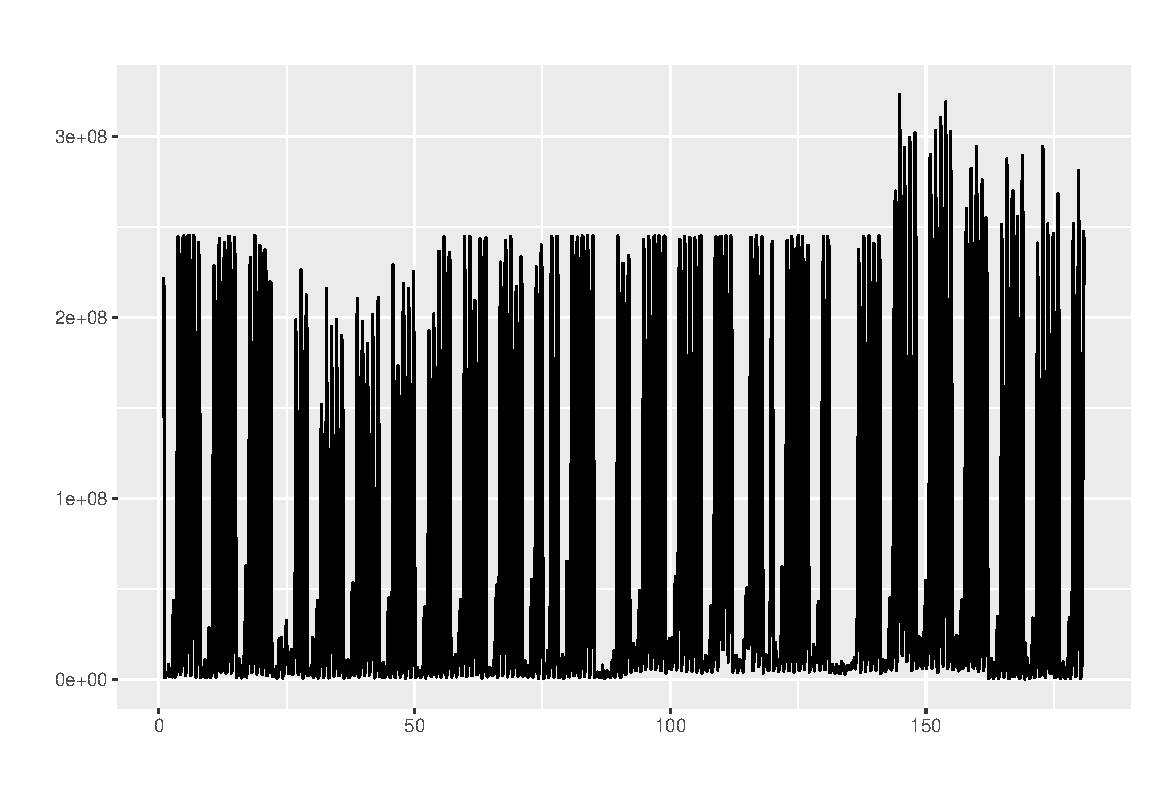
\includegraphics[width=0.7\textwidth,angle=0]{myts_avg_eps.eps}
\end{frame}
%%%%%%%%%%
\subsection{}
\begin{frame}
\frametitle{Proposta}

        \centering
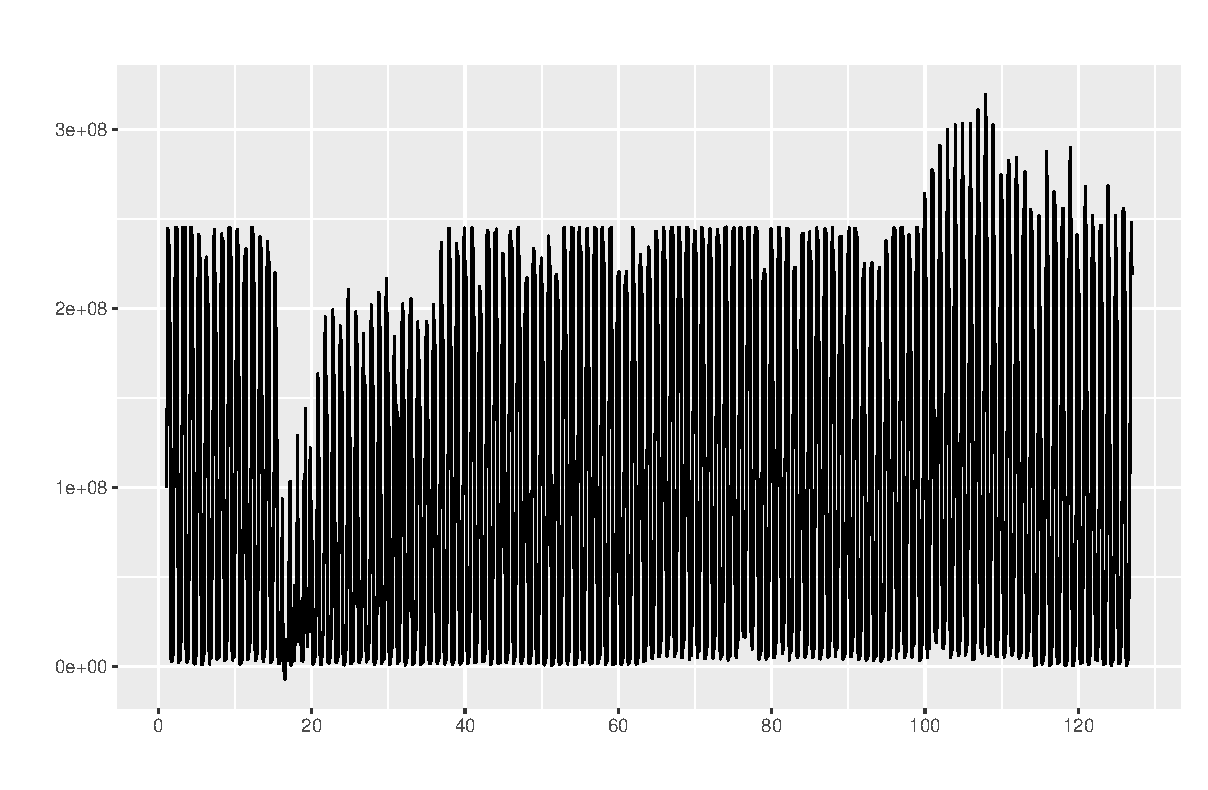
\includegraphics[width=0.7\textwidth,angle=0]{mytsClean.eps}
\end{frame}

\subsection{}
\begin{frame}
\frametitle{Proposta}

        \centering
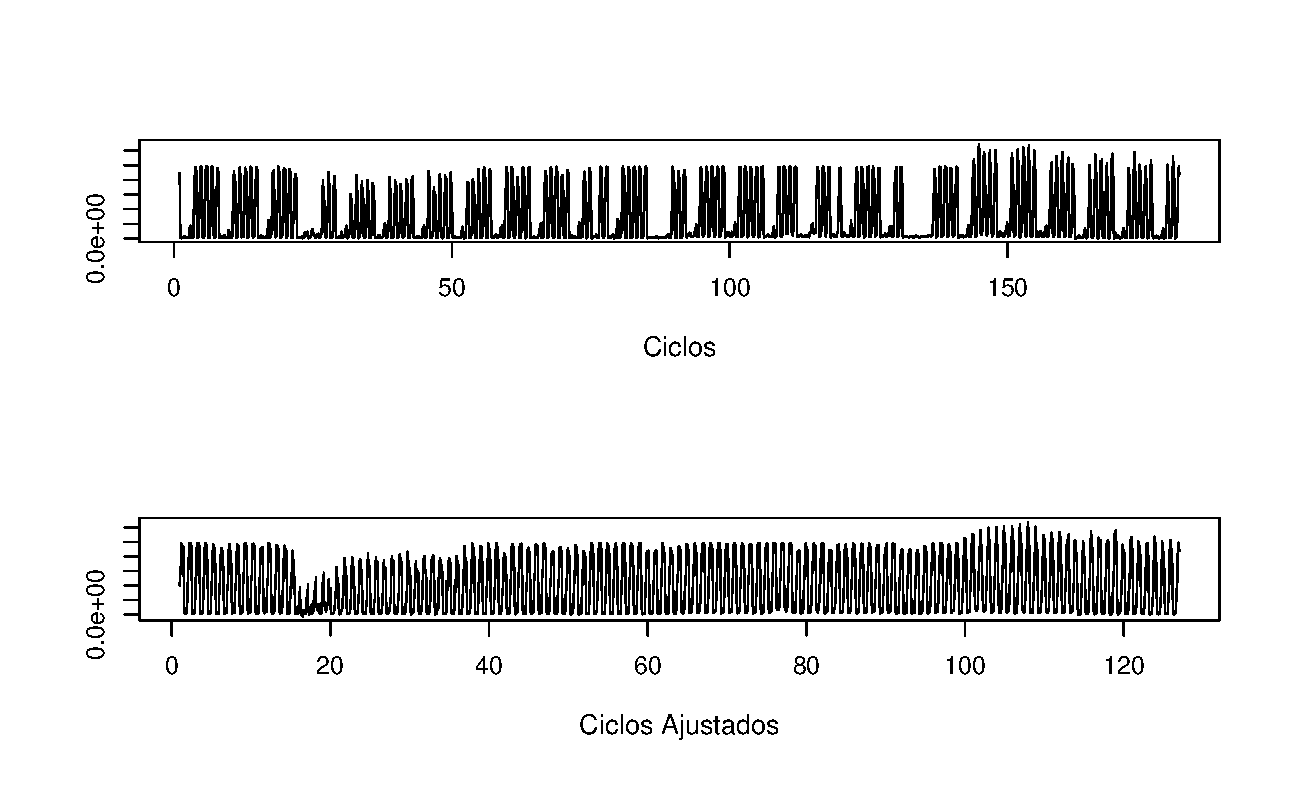
\includegraphics[width=0.75\textwidth,angle=0]{cicloOrig_Ajustado.eps}
\end{frame}
%%%%%%%%%%%%%%%%%%%%%%%%%%%%%%%%%%%%%%
%-------------------------------------
%%%%%%%%%%%%%%%%%%%%%%%%%%%%%%%%%%%%%%
\subsection{}
\begin{frame}
\frametitle{Validação Cruzada}
\small
\begin{block}{Preparando dados para treinamento}
\begin{itemize} \small
    \item Separação dos dados de Ciclos Ajustados.
    \item Um período de 24 horas define um ciclo; portanto, todo o conjunto de dados é composto por 4320 ciclos.
\end{itemize}
\end{block}

\begin{block}{Treinando e testando as amostras}
\begin{itemize} \small
    \item A técnica de Validação Cruzada de Série Temporal (TSCV) foi aplicado aos dados;
    \item O método \textbf{\textit{Hold Out}} foi usado para selecionar os subconjuntos de Treinamento e Teste.
    \item Foi aplicado às primeiras 72 amostras como conjunto de treinamento, às segundas 144 amostras para o treinamento e assim por diante (72, 144, 216,...).
\end{itemize}
\end{block}
\end{frame}
%%%%%%%%%%%%%%%%%%%%%%%%%%%%%%%%%%%%%%
%-------------------------------------
%%%%%%%%%%%%%%%%%%%%%%%%%%%%%%%%%%%%%%

\subsection{}
\begin{frame}
\frametitle{Sequência PRA -- Estacionariedade}
\begin{block}{Execução -- PRA}
    \begin{itemize}
        \item Verificar Comportamento a longo prazo;
        \item Série pode apresentar mudança de nível (inclinações etc.)
        \item Não interferir na capacidade de predição das técnicas;
            \begin{itemize}\setbeamertemplate{itemize items}[triangle]
                \item \textbf{Kwiatkowski-Phillips-Schmidt-Shin} -- (KPSS)
                \item \textbf{Argumented Dickey-Fuller} (DICKEY-FULLER)
                    \begin{itemize}\setbeamertemplate{itemize items}[square]
                    \item Aplicação de direrenciações;
                        \begin{equation}
                             Y_{t} = Z_{t} - Z_{t-1}
                         \end{equation}
                    \end{itemize}
            \end{itemize}
        \end{itemize}
\end{block}
\end{frame}

%%%%%%%%%%%%%%%%%%%%%%%%%%%%%%%%%%%%%%
%-------------------------------------
%%%%%%%%%%%%%%%%%%%%%%%%%%%%%%%%%%%%%%
\section{Resultados}

%%%%%%%%%%%%

\subsection{}
\begin{frame}
\frametitle{Resultados}

\begin{block}{Comparação}
\begin{itemize} \small
    \item O \textbf{PRA} é utilizado como etapa anterior à aplicação da técnica de previsão.
    \item Para medir os benefícios do \textbf{PRA} na capacidade de modelagem e predição das técnicas \textbf{ARIMA} e \textbf{NNAR}, comparamos seu desempenho com e sem a aplicação do mesmo.
    \item A métrica para avaliar a performance da proposta no período \textbf{T} foi a Root Mean Squared Error (RMSE).
\end{itemize}
\end{block}

\begin{block}{\textit{Autocorrelation Function} -
ACF}
\begin{itemize} \small
    \item Aplicado a todos os conjuntos de Treinamento;
    \item Aplicado aos Resíduos;
\end{itemize}
\end{block}
 
\end{frame}

%%%%%%%%%%%%

\subsection{}
\begin{frame}
\frametitle{Results}
\small
\begin{block}{Comparison}
\begin{itemize} \small
    \item The ANP model is used as previous step to the application of the prediction technique.
    \item To measure the benefits of the ANP in the modeling and predition capacity of the ARIMA and NNAR techniques, we compare their performance with and without the application of the ANP model. 
\end{itemize}
\end{block}

\begin{block}{Metric}
\begin{itemize} \small
    \item The metric used to evaluate the performance of the proposal in a period T is the Root Mean Squared Error (RMSE), follows the equation below, where ŷ t is the predicted value and y t is the real values of bandwidth usage in time t.
\end{itemize}

\begin{equation}
RMSE(T) = \frac{1}{\sqrt{T}} (\sum_{t=1}^{T} (\hat{y}_t - y_t)^2)^\frac{1}{2}    
\end{equation}

\end{block}
\end{frame}

%%%%%%%%%%%%

\subsection{}
\begin{frame}
\frametitle{The ANP model improves the performance of prediction techniques}
\small

\begin{itemize}\footnotesize
 \item ARIMA and NNAR reach high values of RSME in several moments, representing the impact of the elastic demand situation in the prediction capacity of both techniques.
 \item When ARIMA and NNAR techniques are applied together with the proposed ANP model, the performance of both techniques increase (lower prediction errors), reaching similar values.
\end{itemize}

\vspace{-0.2cm}

\centering
\begin{figure}[!htb]
\centering
\includegraphics[height=0.37\textwidth,angle=0]{rmse_PRA_original_juntos-eps-converted-to.pdf}
\end{figure}

\end{frame}

%%%%%%%%%%%%

\subsection{}
\begin{frame}
\frametitle{The ANP model favors adaptability to behavioral changes}
\small

\begin{columns}[T] % align columns
\begin{column}{.4\textwidth}
\begin{itemize}\footnotesize
    \item The ANP model can accompany the samples of the time series of the dataset, following the seasonality and amplitude fluctuations, giving the importance of the samples variation (with approximately 2, 4, 6 and 8 weeks)
    \item Moreover, the ANP model reduced the computational processing for the training phase in around 85\% using ARIMA and 12\% applying NNAR. This fact indicates that the ANP model is capable to reduce the processing time for the prediction techniques, enabling its application in real time prediction scenarios.
\end{itemize}
\end{column}%

\hfill%

\begin{column}{.6\textwidth}
\centering
\begin{figure}[!htb]
\centering
\includegraphics[height=0.62\textwidth,angle=0]{melhoresCiclos3_3-eps-converted-to.pdf}
\end{figure}
\end{column}%
\end{columns}

\end{frame}

%%%%%%%%%%%%
%%%%%%%%%%%%%%%%%%%%%%%%%%%%%%%%%%%%%%
%-------------------------------------
%%%%%%%%%%%%%%%%%%%%%%%%%%%%%%%%%%%%%%

\subsection{}
\begin{frame}{Resultados}
    \centering
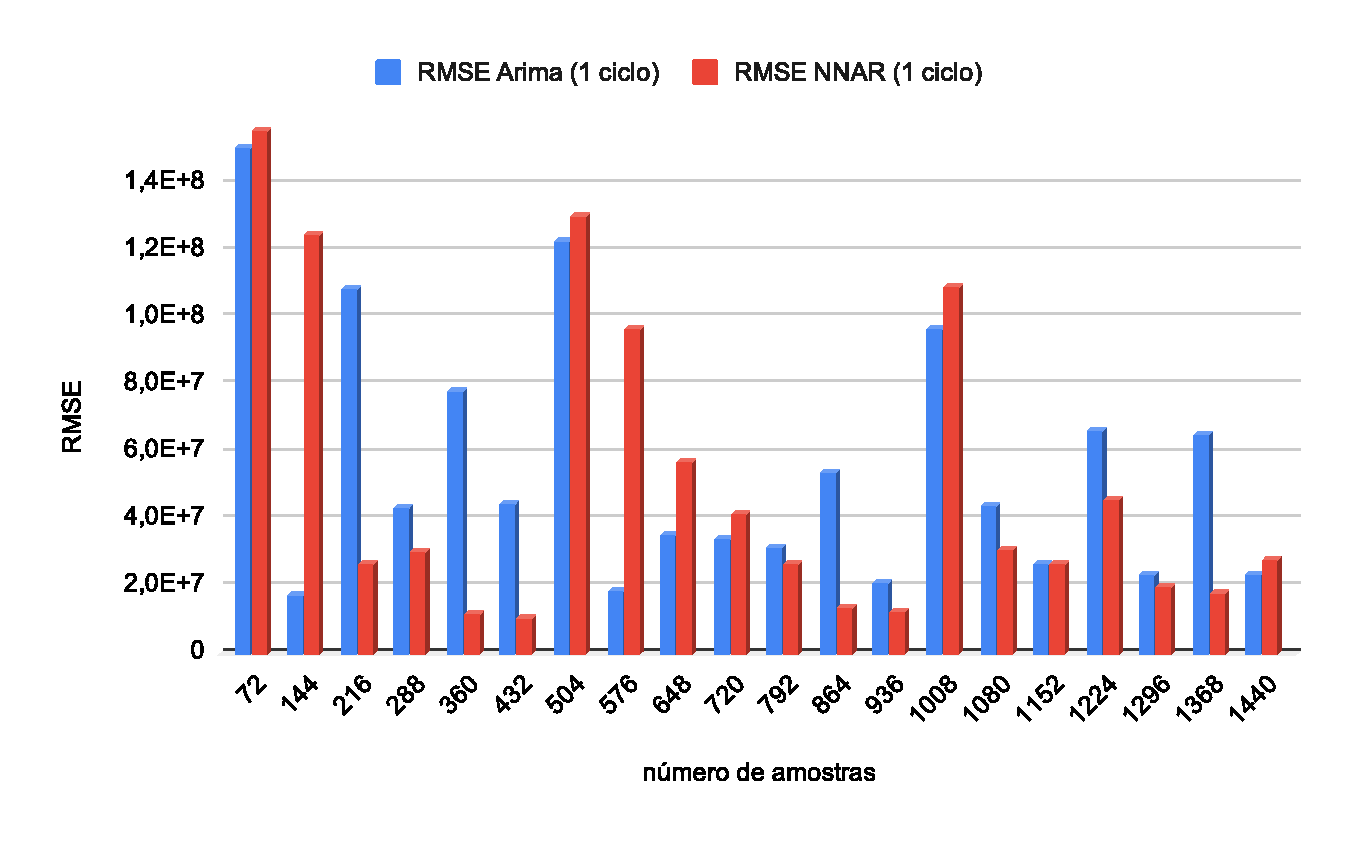
\includegraphics[height=0.50\textwidth,angle=0]{rmse_tsoriginal.eps}
\end{frame}


\subsection{}
\begin{frame}{Resultados}
    \centering
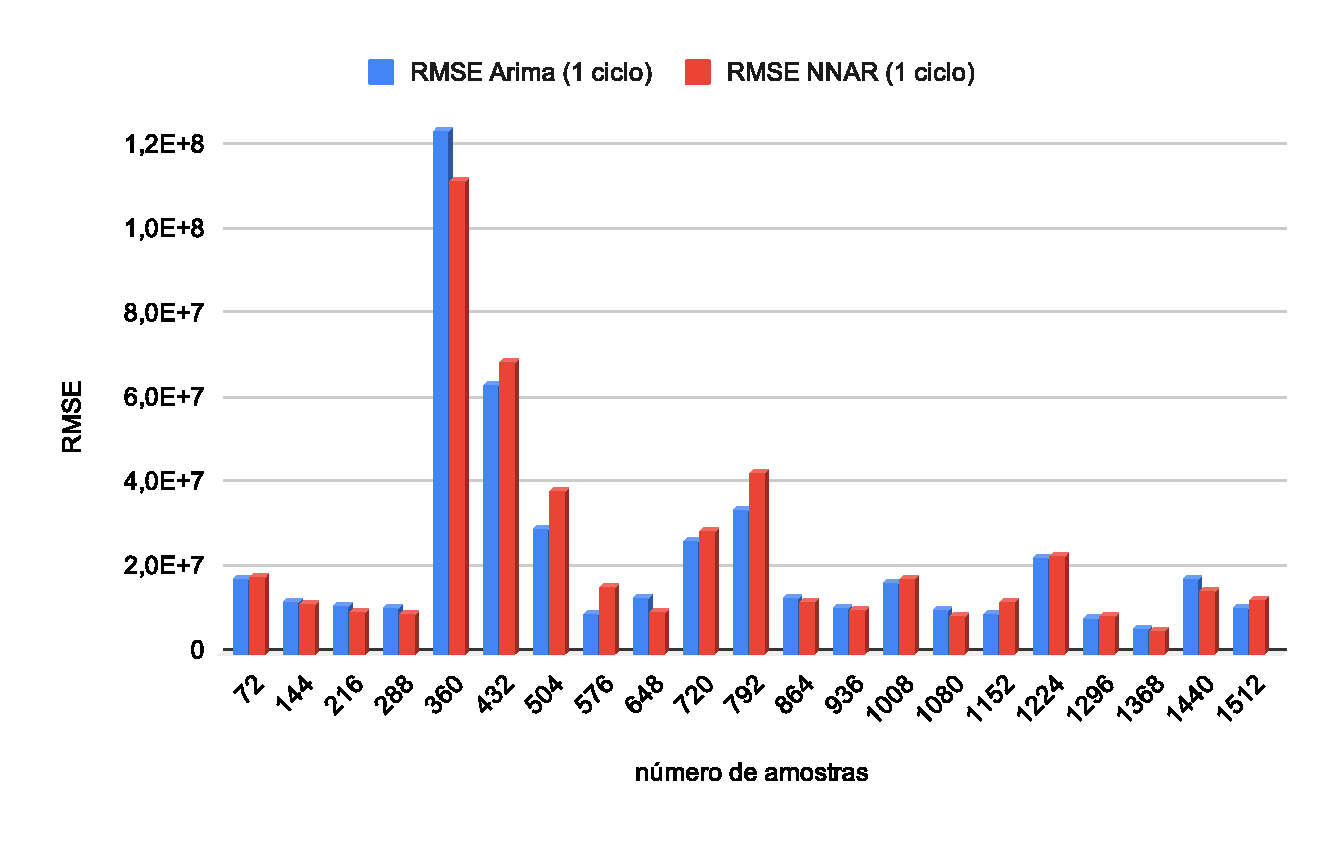
\includegraphics[height=0.50\textwidth,angle=0]{rmse_tsclean.eps}
\end{frame}
%%%%%%%%%%%%%%%%%%%%%%%%%%%%%%%%%%%%%%
%-------------------------------------
%%%%%%%%%%%%%%%%%%%%%%%%%%%%%%%%%%%%%%

%%%%%%%%%%%%

\section{Conclusion}

%%%%%%%%%%%%

\subsection{}
\begin{frame}
\frametitle{Conclusion e Future Work}
\small
\begin{block}{Conclusion}
\begin{itemize} \small
\item The ISPs tend to evolve to MISPs, in order to deal with situations that can affect the QoS of service delivery.
\item Problem: improve the existing prediction techniques, turning them in a efficient approach to overcome situations of elastic demand of network resources.
\item The proposed model, called ANP, is used as previous step to the application of the prediction technique.
\item The experiments performed show that the model ANP together with a prediction technique evolved the prediction capacity, reducing around 30\% the RMSE error rate.
\end{itemize}
\end{block}

\begin{block}{Future Work}
\begin{itemize} \small
\item Extend the prediction approach, including issues related to independent variables, which can generate a higher capacity of knowledge about the elastic demand behavior.
\end{itemize}
\end{block}

\end{frame}

%%%%%%%%%%%%


\subsection{}
\begin{frame}
\frametitle{Obrigado!}
% \small

\begin{block}{Agradecimentos}\small
À banca, examinadora desta apresentação de dissertação de mestrado e ao orientador, Prof. Dr. Rafael Lopes.


\end{block}

\begin{block}{Contato}\small
Email: dyego@larces.uece.br
\end{block}

\end{frame}
%%teste
%%%%%%%%%%%%

\end{document}